\documentclass[11pt,]{article}
\usepackage{lmodern}
\usepackage{amssymb,amsmath}
\usepackage{ifxetex,ifluatex}
\usepackage{fixltx2e} % provides \textsubscript
\ifnum 0\ifxetex 1\fi\ifluatex 1\fi=0 % if pdftex
  \usepackage[T1]{fontenc}
  \usepackage[utf8]{inputenc}
\else % if luatex or xelatex
  \ifxetex
    \usepackage{mathspec}
  \else
    \usepackage{fontspec}
  \fi
  \defaultfontfeatures{Ligatures=TeX,Scale=MatchLowercase}
\fi
% use upquote if available, for straight quotes in verbatim environments
\IfFileExists{upquote.sty}{\usepackage{upquote}}{}
% use microtype if available
\IfFileExists{microtype.sty}{%
\usepackage{microtype}
\UseMicrotypeSet[protrusion]{basicmath} % disable protrusion for tt fonts
}{}
\usepackage[margin=1in]{geometry}
\usepackage{hyperref}
\PassOptionsToPackage{usenames,dvipsnames}{color} % color is loaded by hyperref
\hypersetup{unicode=true,
            pdftitle={A demonstration of combined scientific data processing and publication using Literate Programming in R},
            pdfauthor={Andy Clifton},
            colorlinks=true,
            linkcolor=blue,
            citecolor=cyan,
            urlcolor=red,
            breaklinks=true}
\urlstyle{same}  % don't use monospace font for urls
\usepackage{natbib}
\bibliographystyle{plainnat}
\usepackage{color}
\usepackage{fancyvrb}
\newcommand{\VerbBar}{|}
\newcommand{\VERB}{\Verb[commandchars=\\\{\}]}
\DefineVerbatimEnvironment{Highlighting}{Verbatim}{commandchars=\\\{\}}
% Add ',fontsize=\small' for more characters per line
\usepackage{framed}
\definecolor{shadecolor}{RGB}{248,248,248}
\newenvironment{Shaded}{\begin{snugshade}}{\end{snugshade}}
\newcommand{\AlertTok}[1]{\textcolor[rgb]{0.94,0.16,0.16}{#1}}
\newcommand{\AnnotationTok}[1]{\textcolor[rgb]{0.56,0.35,0.01}{\textbf{\textit{#1}}}}
\newcommand{\AttributeTok}[1]{\textcolor[rgb]{0.77,0.63,0.00}{#1}}
\newcommand{\BaseNTok}[1]{\textcolor[rgb]{0.00,0.00,0.81}{#1}}
\newcommand{\BuiltInTok}[1]{#1}
\newcommand{\CharTok}[1]{\textcolor[rgb]{0.31,0.60,0.02}{#1}}
\newcommand{\CommentTok}[1]{\textcolor[rgb]{0.56,0.35,0.01}{\textit{#1}}}
\newcommand{\CommentVarTok}[1]{\textcolor[rgb]{0.56,0.35,0.01}{\textbf{\textit{#1}}}}
\newcommand{\ConstantTok}[1]{\textcolor[rgb]{0.00,0.00,0.00}{#1}}
\newcommand{\ControlFlowTok}[1]{\textcolor[rgb]{0.13,0.29,0.53}{\textbf{#1}}}
\newcommand{\DataTypeTok}[1]{\textcolor[rgb]{0.13,0.29,0.53}{#1}}
\newcommand{\DecValTok}[1]{\textcolor[rgb]{0.00,0.00,0.81}{#1}}
\newcommand{\DocumentationTok}[1]{\textcolor[rgb]{0.56,0.35,0.01}{\textbf{\textit{#1}}}}
\newcommand{\ErrorTok}[1]{\textcolor[rgb]{0.64,0.00,0.00}{\textbf{#1}}}
\newcommand{\ExtensionTok}[1]{#1}
\newcommand{\FloatTok}[1]{\textcolor[rgb]{0.00,0.00,0.81}{#1}}
\newcommand{\FunctionTok}[1]{\textcolor[rgb]{0.00,0.00,0.00}{#1}}
\newcommand{\ImportTok}[1]{#1}
\newcommand{\InformationTok}[1]{\textcolor[rgb]{0.56,0.35,0.01}{\textbf{\textit{#1}}}}
\newcommand{\KeywordTok}[1]{\textcolor[rgb]{0.13,0.29,0.53}{\textbf{#1}}}
\newcommand{\NormalTok}[1]{#1}
\newcommand{\OperatorTok}[1]{\textcolor[rgb]{0.81,0.36,0.00}{\textbf{#1}}}
\newcommand{\OtherTok}[1]{\textcolor[rgb]{0.56,0.35,0.01}{#1}}
\newcommand{\PreprocessorTok}[1]{\textcolor[rgb]{0.56,0.35,0.01}{\textit{#1}}}
\newcommand{\RegionMarkerTok}[1]{#1}
\newcommand{\SpecialCharTok}[1]{\textcolor[rgb]{0.00,0.00,0.00}{#1}}
\newcommand{\SpecialStringTok}[1]{\textcolor[rgb]{0.31,0.60,0.02}{#1}}
\newcommand{\StringTok}[1]{\textcolor[rgb]{0.31,0.60,0.02}{#1}}
\newcommand{\VariableTok}[1]{\textcolor[rgb]{0.00,0.00,0.00}{#1}}
\newcommand{\VerbatimStringTok}[1]{\textcolor[rgb]{0.31,0.60,0.02}{#1}}
\newcommand{\WarningTok}[1]{\textcolor[rgb]{0.56,0.35,0.01}{\textbf{\textit{#1}}}}
\usepackage{longtable,booktabs}
\usepackage{graphicx,grffile}
\makeatletter
\def\maxwidth{\ifdim\Gin@nat@width>\linewidth\linewidth\else\Gin@nat@width\fi}
\def\maxheight{\ifdim\Gin@nat@height>\textheight\textheight\else\Gin@nat@height\fi}
\makeatother
% Scale images if necessary, so that they will not overflow the page
% margins by default, and it is still possible to overwrite the defaults
% using explicit options in \includegraphics[width, height, ...]{}
\setkeys{Gin}{width=\maxwidth,height=\maxheight,keepaspectratio}
\IfFileExists{parskip.sty}{%
\usepackage{parskip}
}{% else
\setlength{\parindent}{0pt}
\setlength{\parskip}{6pt plus 2pt minus 1pt}
}
\setlength{\emergencystretch}{3em}  % prevent overfull lines
\providecommand{\tightlist}{%
  \setlength{\itemsep}{0pt}\setlength{\parskip}{0pt}}
\setcounter{secnumdepth}{5}
% Redefines (sub)paragraphs to behave more like sections
\ifx\paragraph\undefined\else
\let\oldparagraph\paragraph
\renewcommand{\paragraph}[1]{\oldparagraph{#1}\mbox{}}
\fi
\ifx\subparagraph\undefined\else
\let\oldsubparagraph\subparagraph
\renewcommand{\subparagraph}[1]{\oldsubparagraph{#1}\mbox{}}
\fi

%%% Use protect on footnotes to avoid problems with footnotes in titles
\let\rmarkdownfootnote\footnote%
\def\footnote{\protect\rmarkdownfootnote}

%%% Change title format to be more compact
\usepackage{titling}

% Create subtitle command for use in maketitle
\providecommand{\subtitle}[1]{
  \posttitle{
    \begin{center}\large#1\end{center}
    }
}

\setlength{\droptitle}{-2em}

  \title{A demonstration of combined scientific data processing and publication using Literate Programming in R}
    \pretitle{\vspace{\droptitle}\centering\huge}
  \posttitle{\par}
    \author{Andy Clifton}
    \preauthor{\centering\large\emph}
  \postauthor{\par}
      \predate{\centering\large\emph}
  \postdate{\par}
    \date{2019-10-17}


\begin{document}
\maketitle

{
\hypersetup{linkcolor=black}
\setcounter{tocdepth}{2}
\tableofcontents
}
\hypertarget{introduction}{%
\section{Introduction}\label{introduction}}

something something reproducible research, mumble, grumble, get off my lawn, grumble

\hypertarget{linking-analysis-and-publication-workflows}{%
\subsection{Linking analysis and publication workflows}\label{linking-analysis-and-publication-workflows}}

Anecdotally, the separation of the publication from the analysis process has been a barrier to reproducible research, as it is impossible to ensure the link between source data and final publication.

This document demonstrates the concept of Literate Programming. Literate programming means that the program documentation is complete and contained within the program itself. It is important to note that the documentation is effectively a publication, and thus it is possible to combine data analysis with the creation of a publication in the same file. The use of literate programming therefore mitigates this barrier to reproducible research.

Furthermore, this project has been structured so that the data required for this publication are in a subdirectory of the project. This means that all of the files required to reproduce the analysis results can be included in a repository.

\hypertarget{how-literate-programming-was-used-to-write-this-document}{%
\subsection{How Literate Programming was used to write this document}\label{how-literate-programming-was-used-to-write-this-document}}

In this example, an output PDF document and results are generated from a file called \emph{main.rmd}. \emph{main.rmd} is an \href{https://rmarkdown.rstudio.com/authoring_basics.html}{R markdown file}. R markdown is a flavor of markdown that can be processed by the R programming language \citep{R-base} to run code (i.e, do analysis) and create documentation from the same document. This is done using a package called \emph{knitr}. Instructions for how to run \emph{knitr} are included in the \emph{howto.md} file in this repository. A far more detailed guide to writing using R markdown can be found in \citet{R-Markdown-Guide}.

The markdown document contains a mixture of documentation and so-called ``code chunks''. The code chunks can be configured so that their outputs are echoed to the document (or not), which in turn allows the output PDF to show only those parts of the data processing that are relevant.

I suggest reading this PDF together with the R markdown file (\emph{main.rmd}) and possibly the \emph{knitr} instructions \footnote{See \url{https://yihui.name/knitr/}}. This will greatly help in understanding what is done in the processing and what makes it to the publication.

\hypertarget{but-i-hate-r}{%
\subsection{But I hate R}\label{but-i-hate-r}}

You don't mean that. But just in case you can't handle learning yet another new language, this next statement might interest you.

\begin{quote}
``A less well-known fact about R Markdown is that many other languages are also supported, such as Python, Julia, C++, and SQL. The support comes from the knitr package, which has provided a large number of language engines.''"

--- \citet{R-Markdown-Guide}
\end{quote}

The currently available language engines are:

\begin{Shaded}
\begin{Highlighting}[]
\KeywordTok{names}\NormalTok{(knitr}\OperatorTok{::}\NormalTok{knit_engines}\OperatorTok{$}\KeywordTok{get}\NormalTok{())}
\end{Highlighting}
\end{Shaded}

\begin{verbatim}
##  [1] "awk"         "bash"        "coffee"      "gawk"        "groovy"     
##  [6] "haskell"     "lein"        "mysql"       "node"        "octave"     
## [11] "perl"        "psql"        "Rscript"     "ruby"        "sas"        
## [16] "scala"       "sed"         "sh"          "stata"       "zsh"        
## [21] "highlight"   "Rcpp"        "tikz"        "dot"         "c"          
## [26] "fortran"     "fortran95"   "asy"         "cat"         "asis"       
## [31] "stan"        "block"       "block2"      "js"          "css"        
## [36] "sql"         "go"          "python"      "julia"       "sass"       
## [41] "scss"        "theorem"     "lemma"       "corollary"   "proposition"
## [46] "conjecture"  "definition"  "example"     "exercise"    "proof"      
## [51] "remark"      "solution"
\end{verbatim}

So, you have no excuse. You can simply write your code in any of the 52 languages, and off you go.

\hypertarget{implementing-a-coupled-analysis-and-publication-workflow}{%
\section{Implementing a coupled analysis and publication workflow}\label{implementing-a-coupled-analysis-and-publication-workflow}}

An analysis and publication workflow usually follows a similar path:

\begin{enumerate}
\def\labelenumi{\arabic{enumi}.}
\tightlist
\item
  Set up the computing environment
\item
  Load our own data processing routines
\item
  Import data
\item
  Plot it
\item
  Do some operations
\item
  Plot some more
\item
  Write.
\item
  Format for a journal
\item
  Iterate around items 1-9 for a while
\item
  Submit
\end{enumerate}

Fortunately, all of this can be captured in a markdown document.

\hypertarget{setting-up-the-computing-environment}{%
\subsection{Setting up the computing environment}\label{setting-up-the-computing-environment}}

Like most scripts, \emph{main.rmd} includes a few variables that the user must set to run the analysis.

\begin{itemize}
\tightlist
\item
  The \emph{project.root} variable defines the location of the files required for this analysis.
\item
  The \emph{made.by} variable forms part of a label that will be added to the plots.
\end{itemize}

An advantage of \emph{knitr} is that we can simply execute the code and show the code and results inline:

\begin{Shaded}
\begin{Highlighting}[]
\CommentTok{# Where can files be found?}
\NormalTok{project.root <-}\StringTok{ }\KeywordTok{file.path}\NormalTok{(}\StringTok{'/Users/andyc/Documents/public/GitHub/LiterateDemo'}\NormalTok{)}
\NormalTok{project.root}

\CommentTok{# Who ran this script}
\NormalTok{made.by =}\StringTok{ "A. Clifton"}
\NormalTok{made.by}
\end{Highlighting}
\end{Shaded}

\begin{verbatim}
## [1] "/Users/andyc/Documents/public/GitHub/LiterateDemo"
## [1] "A. Clifton"
\end{verbatim}

We can also show the value of those variables in the documentation using backticks around the variable names in the markdown.

\begin{itemize}
\tightlist
\item
  \emph{project.root} is /Users/andyc/Documents/public/GitHub/LiterateDemo
\item
  \emph{made.by} is A. Clifton.
\end{itemize}

We want to change our working directory (\emph{working.dir} ) to the root directory of the project. We've already set up several important subdirectories:

\begin{itemize}
\tightlist
\item
  /\textbf{code} contains functions required for the analysis
\item
  /\textbf{data} contains the data files to be analyzed.
\end{itemize}

Let's tell the code where these are.

We'll also create a new directory for the results of the analysis. In this case it can be found at \textbf{/Users/andyc/Documents/public/GitHub/LiterateDemo/analysis/all}.

\textbf{Note:} Packages are required to supplement base functions in R and many other languages. For example, this script requires the \emph{bookdown}, \emph{ggplot2}, \emph{grid}, \emph{knitr}, \emph{RColorBrewer}, \emph{rgdal}, and \emph{stringr} packages to run. These are called from the script using the \emph{require()} function. This assumes that the packaages are available on your system.\footnote{For details of how to install packages, see the RStudio help.} The use of packages represents a challenge to reproducable and repeatable research as it is possible that the function and output of the packages may change over time.

\hypertarget{loading-our-own-routines}{%
\subsection{Loading our own routines}\label{loading-our-own-routines}}

Every data processing workflow requires its own scripts or functions to run. In this example, they are included in the \emph{codes} directory and sourced during the preparation of this document. I have included output below to show these codes being called.

\begin{Shaded}
\begin{Highlighting}[]
\CommentTok{# source these functions}
\NormalTok{code.files =}\StringTok{ }\KeywordTok{dir}\NormalTok{(code.dir, }\DataTypeTok{pattern =} \StringTok{"}\CharTok{\textbackslash{}\textbackslash{}}\StringTok{.R$"}\NormalTok{)}
\ControlFlowTok{for}\NormalTok{ (file }\ControlFlowTok{in}\NormalTok{ code.files)\{}
  \KeywordTok{source}\NormalTok{(}\DataTypeTok{file =} \KeywordTok{file.path}\NormalTok{(code.dir,file))}
  \KeywordTok{print}\NormalTok{(}\KeywordTok{paste0}\NormalTok{(}\StringTok{"Sourcing "}\NormalTok{, file, }\StringTok{"."}\NormalTok{))}
\NormalTok{\}}
\end{Highlighting}
\end{Shaded}

\begin{verbatim}
## [1] "Sourcing cleanPlot.R."
## [1] "Sourcing plotInfoLabel.R."
## [1] "Sourcing plotSomething.R."
## [1] "Sourcing theme_Literate.R."
\end{verbatim}

\hypertarget{load-the-data}{%
\subsection{Load the data}\label{load-the-data}}

We now analyse the data from the simple data set. In this case, code has been written to load all of the files in the \emph{data.dir} directory (/Users/andyc/Documents/public/GitHub/LiterateDemo/data). I'm also going to map the three columns in the data files to the variables \(x\), \(y\), and \(z\).\footnote{See \url{https://www.calvin.edu/~rpruim/courses/s341/S17/from-class/MathinRmd.html} for more information about including maths in R markdown}

\hypertarget{plot-input-data}{%
\subsection{Plot input data}\label{plot-input-data}}

The next step is to plot the input data. In this case we plot all of the input data together in one plot, but there are many different possibilities. Figures can also be given a consistent look and feel through ggplot's themes.

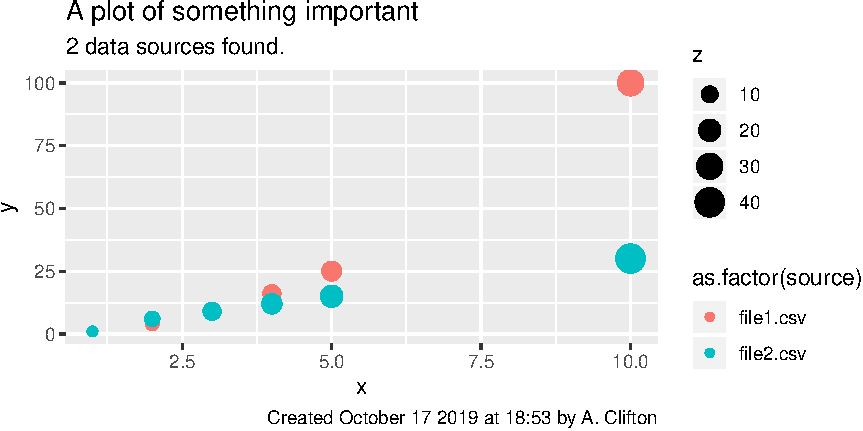
\includegraphics{main_files/figure-latex/plot input data-1.pdf}

For convenience, we'll also save a copy of the figure as a \emph{.png} file to the \emph{analysis} directory.

\hypertarget{operate-on-the-data}{%
\subsection{Operate on the data}\label{operate-on-the-data}}

At this point we can do any number of operations on the data. For sake of demonstration, let's add 2 to all \(x\) values.

\begin{Shaded}
\begin{Highlighting}[]
\NormalTok{df.all <-}\StringTok{ }\NormalTok{df.in}
\NormalTok{df.all}\OperatorTok{$}\NormalTok{x <-}\StringTok{ }\NormalTok{df.in}\OperatorTok{$}\NormalTok{x }\OperatorTok{+}\StringTok{ }\FloatTok{2.0}
\end{Highlighting}
\end{Shaded}

\hypertarget{plot-the-results}{%
\subsection{Plot the results}\label{plot-the-results}}

Let's run that \emph{plotSomething} routine again.

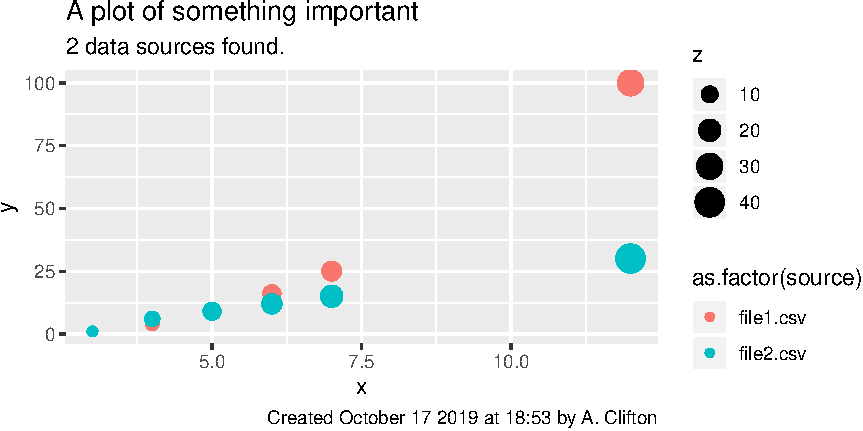
\includegraphics{main_files/figure-latex/plot modified data-1.pdf}

And, as we can see, the data have shifted along \(x\) by a small amount.

\hypertarget{connect-processing-with-publication}{%
\subsection{Connect processing with publication}\label{connect-processing-with-publication}}

So far we have demonstrate that we can import and manipulate data and plot results. Another important part of a publication is the ability to generate statistics or summary information from data and include that in our text.

To demonstrate that, I can calculate that the maximum value of \(y\) in the input data sets was 100. This can be confirmed by checking the input data files. I could also include more complex logic in these statements, for example to say if one statistic is bigger or larger than another.

We sometimes need to include formatted tables in documents. This can be done using the \emph{kable} function (Table \ref{tab:dfall}).

\begin{Shaded}
\begin{Highlighting}[]
\NormalTok{knitr}\OperatorTok{::}\KeywordTok{kable}\NormalTok{(df.all,}
             \DataTypeTok{booktabs=}\OtherTok{TRUE}\NormalTok{,}
             \DataTypeTok{caption =} \StringTok{"The df.all data frame."}\NormalTok{)}
\end{Highlighting}
\end{Shaded}

\begin{table}[t]

\caption{\label{tab:dfall}The df.all data frame.}
\centering
\begin{tabular}{rrrl}
\toprule
x & y & z & source\\
\midrule
3 & 1 & 3 & file1.csv\\
4 & 4 & 6 & file1.csv\\
5 & 9 & 9 & file1.csv\\
6 & 16 & 12 & file1.csv\\
7 & 25 & 15 & file1.csv\\
\addlinespace
12 & 100 & 30 & file1.csv\\
3 & 1 & 4 & file2.csv\\
4 & 6 & 8 & file2.csv\\
5 & 9 & 12 & file2.csv\\
6 & 12 & 16 & file2.csv\\
\addlinespace
7 & 15 & 20 & file2.csv\\
12 & 30 & 40 & file2.csv\\
\bottomrule
\end{tabular}
\end{table}

\hypertarget{save-the-processed-data}{%
\subsection{Save the processed data}\label{save-the-processed-data}}

We now write our processed data to file.

\begin{Shaded}
\begin{Highlighting}[]
\CommentTok{# save the data}
\KeywordTok{save}\NormalTok{(}\DataTypeTok{list =} \KeywordTok{c}\NormalTok{(}\StringTok{"project.root"}\NormalTok{,}
              \StringTok{"made.by"}\NormalTok{,}
              \StringTok{"df.all"}\NormalTok{),}
       \DataTypeTok{file =} \KeywordTok{file.path}\NormalTok{(output.dir,}\StringTok{"Data.RData"}\NormalTok{),}
       \DataTypeTok{envir =}\NormalTok{ .GlobalEnv)}
\end{Highlighting}
\end{Shaded}

In R it is also possible to save the whole workspace. We can do that here as well:

\begin{Shaded}
\begin{Highlighting}[]
\CommentTok{# save the workspace}
\KeywordTok{save.image}\NormalTok{(}\DataTypeTok{file=}\KeywordTok{file.path}\NormalTok{(output.dir,}\StringTok{"workspace.RData"}\NormalTok{))}
\end{Highlighting}
\end{Shaded}

\hypertarget{saving-packages}{%
\subsection{Saving packages}\label{saving-packages}}

\hypertarget{applying-journal-formating}{%
\subsection{Applying Journal formating}\label{applying-journal-formating}}

Scientific Journals often have their own formatting requirements. These requirements can still be met using markdown. The mechanics of such a process are beyond the scope of this paper and should probably be done as the last step in the publishing process. The reader is suggested to look at the \emph{rticles} package and to use the detailed instructions in section 13 of the R Markdown Guide \citep{R-Markdown-Guide}.

\hypertarget{conclusions}{%
\section{Conclusions}\label{conclusions}}

It is possible to write a single document that captures all of the process of preparing and analysing data and creating a publication to describe that data.

\bibliography{main.bib}


\end{document}
